\chapter{Prezentacja warstwy użytkowej projektu}
Po utworzeniu i testach projektu przeprowadzona została weryfikacja działania projektu, w celu sprawdzenia poprawności funkcjonowania projektu zgodnie z zasadami założonymi w poprzednich rozdziałach. Poniżej przedstawione są efekty działania warstywy konsolowej projektu w postaci "Print screen-ów". Jest to kilka wybranych operacji które może wykonać użytkownik aplikacji.

Pierwsze zdjęcie przedstawia główne menu aplikacji, gdzie możemy wybrać interesujący nas tryb.
\begin{center}
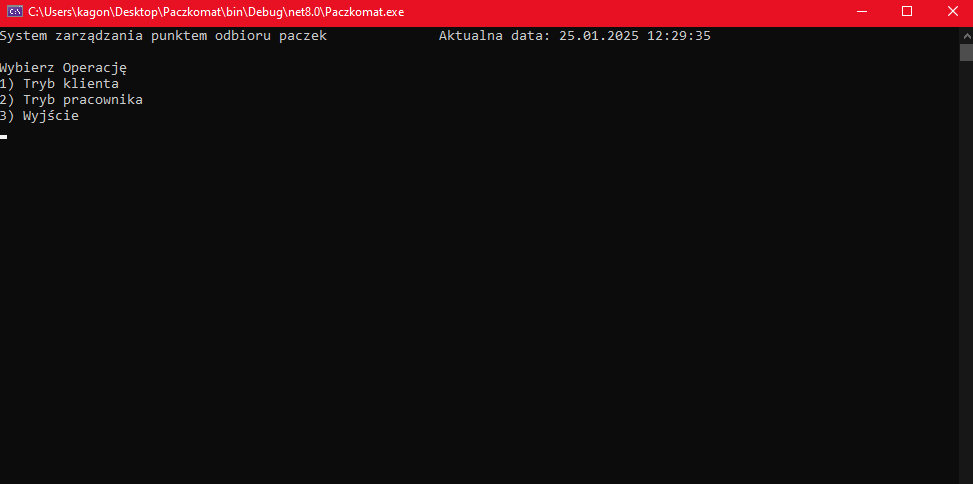
\includegraphics[width=13.0cm, height=8.0cm]{Menu projekt.png}
\end{center}

Następnie wybieramy tryb pracownika, a dokładniej kuriera, gdzie wykonamy operacje takie jak:
Nadanie paczki:
\begin{center}
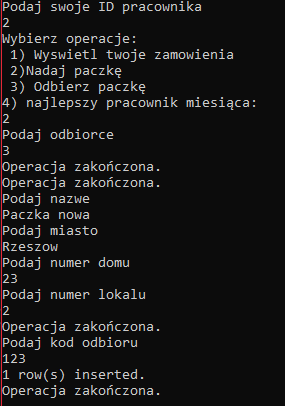
\includegraphics[width=13.0cm, height=13.0cm]{Nadanie paczki kurier.png}
\end{center}

Wyświetlenie zamówień obsługiwanych przez podanego kuriera:
\begin{center}
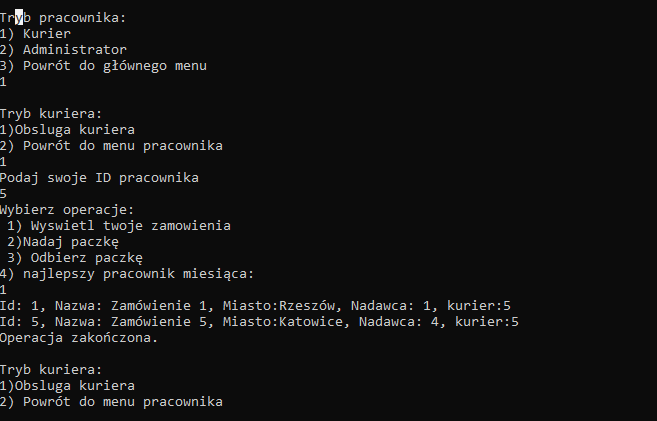
\includegraphics[width=13.0cm, height=7.0cm]{kurier moje zamowienia.png}
\end{center}

Następnie przechodzimy do trybu administratora i jego weryfikacji. Po weryfikacji admin ma możliwość wykonania 6 operacji:
\begin{center}
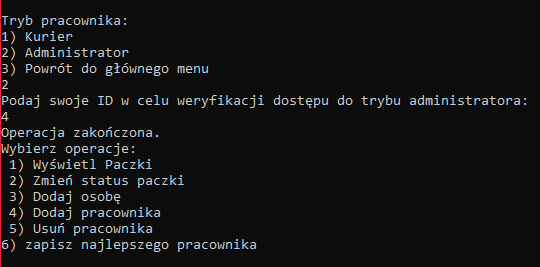
\includegraphics[width=13.0cm, height=3.0cm]{weryfikacja kurier.png}
\end{center}

W trybie klienta możemy wyświetlić nasze przesyłki oraz informacje naszego profilu.
\begin{center}
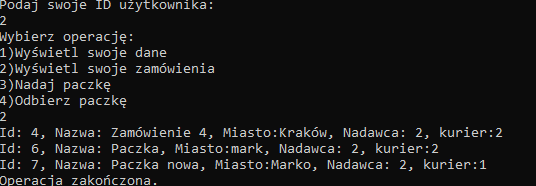
\includegraphics[width=13.0cm, height=3.0cm]{Klient moje paczki.png}
\end{center}
\begin{center}
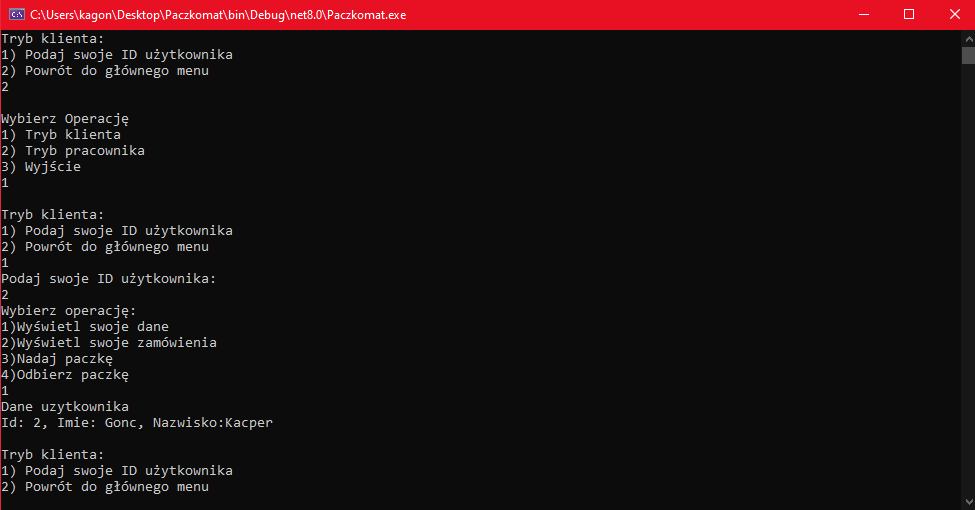
\includegraphics[width=13.0cm, height=8.0cm]{Klient informacje osoby.png}
\end{center}

Aby dokonać odebrania paczki z paczkomatu, klient musi podać ID paczki, jak również kod weryfikacyjny w postaci kodu odbioru.
\begin{center}
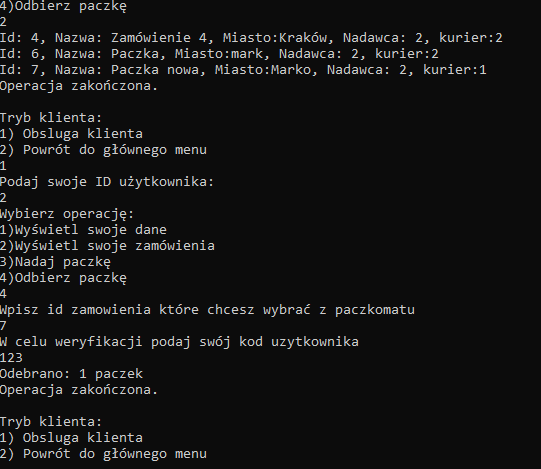
\includegraphics[width=13.0cm, height=5.0cm]{Odbior klienta.png}
\end{center}
